% datastruct/datastruct.tex

\QuickQuizChapter{chp:Data Structures}{Data Structures}

Efficient access to data is critically important to performance, and
therefore discussions of algorithms therefore focus heavily on the
time complexity of the related
data structures~\cite{ThomasHCorman2001Algorithms}.
However, for parallel programs, measures of time complexity must also
include the effects of concurrency.
These concurrency effects can be overwhelmingly large, as discussed in
Chapter~\ref{chp:Hardware and its Habits}, which means that design of
concurrent data structures must pay at least as much attention to the
concurrency effects as it does to the classical sequential time
complexity.

As discussed in Chapter~\ref{cha:Partitioning and Synchronization Design},
an excellent way to achieve high scalability is partitioning.
This points the way to partitionable data structures, a topic taken up by
Section~\ref{sec:datastruct:Partitionable Data Structures}.
Chapter~\ref{chp:Deferred Processing} described how deferring some
actions can greatly improve both performance and scalability.
Section~\ref{sec:defer:Read-Copy Update (RCU)} in particular showed
how to tap the awesome power of procrastination in pursuit of
performance and scalability, a topic take up by
Section~\ref{sec:datastruct:Read-Mostly Data Structures}.

Sometimes scalability is not the goal, for example, when the design
arranges for a given data structure's concurrency to be contrained
to very low levels, but where concurrent access is nevertheless
possible, a possibility raised near the end of
Section~\ref{sec:SMPdesign:Double-Ended Queue Discussion}.
This situation requires data structures that do not necessarily scale
well, but which perform well and which tolerate concurrent access
without failure, a topic taken up by
Section~\ref{sec:datastruct:Concurrency-Tolerant Data Structures}.

Although the best performance and scalability results design rather
than after-the-fact micro-optimization, it is nevertheless the case
that micro-optimization has an important place in achieving the
absolute best possible performance and scalability.
This topic is therefore taken up in
Section~\ref{sec:datastruct:Micro-Optimization}.

Finally, Section~\ref{sec:datastruct:Summary}
presents a summary of this chapter.

\section{Partitionable Data Structures}
\label{sec:datastruct:Partitionable Data Structures}

Chapter~\ref{cha:Partitioning and Synchronization Design}
emphasized the need to apply partitioning in order to attain
respectable performance and scalability, so partitionability
must be a first-class criterion when selecting data structures.
This criterion is well satisfied by that workhorse of parallelism,
the hash table.
Hash tables are conceptually simple, consisting of an array of
\emph{hash buckets}.
A \emph{hash function} maps from a given element's \emph{key}
to the hash bucket that this element will be stored in.
Each hash bucket therefore heads up a linked list of elements,
called a \emph{hash chain}.
When properly configured, these hash chains will be quite short,
permitting a hash table to access the element with a given key
extremely efficiently.

\QuickQuiz{}
	But there are many types of hash tables, of which the chained
	hash tables described here are but one type.
	Why the focus on chained hash tables?
\QuickQuizAnswer{
	Chained hash tables are completely partitionable, and thus
	well-suited to concurrent use.
	There are other completely-partitionable hash tables, for
	example, split-ordered list~\cite{OriShalev2006SplitOrderListHash},
	but they are considerably more complex.
	We therefore start with chained hash tables.
} \QuickQuizEnd

In addition, each bucket can be given its own lock, so that
elements in different buckets of the hash table may be added,
deleted, and looked up completely independently.
A large hash table containing a large number of elements therefore
offers excellent scalability.

\begin{figure}[tb]
{ \scriptsize
\begin{verbatim}
  1 struct ht_elem {
  2   struct cds_list_head hte_next;
  3   unsigned long hte_hash;
  4 };
  5 
  6 struct ht_bucket {
  7   struct cds_list_head htb_head;
  8   spinlock_t htb_lock;
  9 };
 10 
 11 struct hashtab {
 12   unsigned long ht_nbuckets;
 13   struct ht_bucket ht_bkt[0];
 14 };
\end{verbatim}
}
\caption{Hash-Table Data Structures}
\label{fig:datastruct:Hash-Table Data Structures}
\end{figure}

\begin{figure}[tb]
\begin{center}
\resizebox{3in}{!}{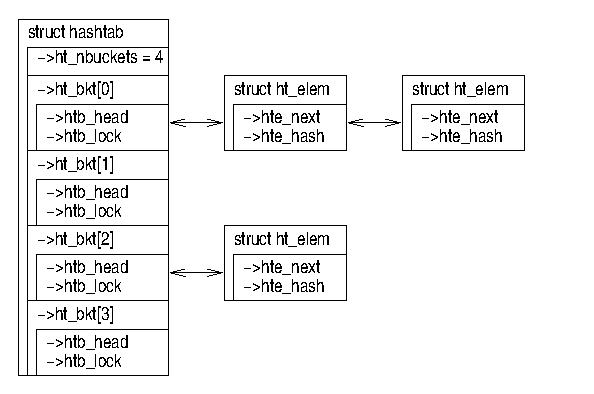
\includegraphics{datastruct/hashdiagram}}
\end{center}
\caption{Hash-Table Data-Structure Diagram}
\label{fig:datastruct:Hash-Table Data-Structure Diagram}
\end{figure}

Figure~\ref{fig:datastruct:Hash-Table Data Structures}
(\co{hash_bkt.c})
shows a set of data structures used in a simple fixed-sized hash
table using chaining and per-hash-bucket locking, and
Figure~\ref{fig:datastruct:Hash-Table Data-Structure Diagram}
diagrams how they fit together.
The \co{hashtab} structure (lines~11-14 in
Figure~\ref{fig:datastruct:Hash-Table Data Structures})
contains four \co{ht_bucket} structures (lines~6-9
Figure~\ref{fig:datastruct:Hash-Table Data Structures}),
with the \co{->bt_nbuckets} field controlling the number of buckets.
Each such bucket contains a list header \co{->htb_head} and
a lock \co{->htb_lock}.
The list headers chain \co{ht_elem} structures
(lines~1-4 in
Figure~\ref{fig:datastruct:Hash-Table Data Structures})
through their
\co{->hte_next} fields, and each \co{ht_elem} structure also caches
the corresponding element's hash value in the \co{->hte_hash} field.
The \co{ht_elem} structure would be included in the larger structure
being placed in the hash table, and this larger structure might contain
a complex key.

The diagram shown in
Figure~\ref{fig:datastruct:Hash-Table Data-Structure Diagram}
has bucket~0 with two elements and bucket~2 with one.

\begin{figure}[tb]
{ \scriptsize
\begin{verbatim}
  1 #define HASH2BKT(htp, h) \
  2   (&(htp)->ht_bkt[h % (htp)->ht_nbuckets])
  3 
  4 static void hashtab_lock(struct hashtab *htp,
  5                          unsigned long hash)
  6 {
  7   spin_lock(&HASH2BKT(htp, hash)->htb_lock);
  8 }
  9 
 10 static void hashtab_unlock(struct hashtab *htp,
 11                            unsigned long hash)
 12 {
 13   spin_unlock(&HASH2BKT(htp, hash)->htb_lock);
 14 }
\end{verbatim}
}
\caption{Hash-Table Mapping and Locking}
\label{fig:datastruct:Hash-Table Mapping and Locking}
\end{figure}

Figure~\ref{fig:datastruct:Hash-Table Mapping and Locking}
shows mapping and locking functions.
Lines~1 and~2 show the macro \co{HASH2BKT()}, which maps from a hash value
to the corresponding \co{ht_bucket} structure.
This macro uses a simple modulus: if more aggressive hashing is required,
the caller needs to implement it when mapping from key to hash value.
The remaining two functions acquire and release the \co{->htb_lock}
corresponding to the specified hash value.

\begin{figure}[tb]
{ \scriptsize
\begin{verbatim}
  1 struct ht_elem *
  2 hashtab_lookup(struct hashtab *htp,
  3                unsigned long hash,
  4                void *key,
  5                int (*cmp)(struct ht_elem *htep,
  6                           void *key))
  7 {
  8   struct ht_bucket *htb;
  9   struct ht_elem *htep;
 10 
 11   htb = HASH2BKT(htp, hash);
 12   cds_list_for_each_entry(htep,
 13                           &htb->htb_head,
 14                           hte_next) {
 15     if (htep->hte_hash != hash)
 16       continue;
 17     if (cmp(htep, key))
 18       return htep;
 19   }
 20   return NULL;
 21 }
\end{verbatim}
}
\caption{Hash-Table Lookup}
\label{fig:datastruct:Hash-Table Lookup}
\end{figure}

Figure~\ref{fig:datastruct:Hash-Table Lookup}
shows \co{hashtab_lookup()},
which returns a pointer to the element with the specified hash and key if it
exists, or \co{NULL} otherwise.
This function takes both a hash value and a pointer to the key because
this allows users of this function to use arbitrary keys and
arbitrary hash functions, with the key-comparison function passed in via
\co{cmp()}, in a manner similar to \co{qsort()}.
Line~11 maps from the hash value to a pointer to the corresponding
hash bucket.
Each pass through the loop spanning line~12-19 examines one element
of the bucket's hash chain.
Line~15 checks to see if the hash values match, and if not, line~16
proceeds to the next element.
Line~17 checks to see if the actual key matches, and if so,
line~18 returns a pointer to the matching element.
If no element matches, line~20 returns \co{NULL}.

\QuickQuiz{}
	But isn't the double comparison on lines~15-18 in
	Figure~\ref{fig:datastruct:Hash-Table Lookup} inefficient
	in the case where the key fits into an unsigned long?
\QuickQuizAnswer{
	Indeed it is!
	However, hash tables quite frequently store information with
	keys such as character strings that do not necessarily fit
	into an unsigned long.
	Simplifying the hash-table implementation for the case where
	keys always fit into unsigned longs is left as an exercise
	for the reader.
} \QuickQuizEnd

\begin{figure}[tb]
{ \scriptsize
\begin{verbatim}
  1 void
  2 hashtab_add(struct hashtab *htp,
  3             unsigned long hash,
  4             struct ht_elem *htep)
  5 {
  6   htep->hte_hash = hash;
  7   cds_list_add(&htep->hte_next,
  8                &HASH2BKT(htp, hash)->htb_head);
  9 }
 10 
 11 void hashtab_del(struct ht_elem *htep)
 12 {
 13   cds_list_del_init(&htep->hte_next);
 14 }
\end{verbatim}
}
\caption{Hash-Table Modification}
\label{fig:datastruct:Hash-Table Modification}
\end{figure}

Figure~\ref{fig:datastruct:Hash-Table Modification}
shows the \co{hashtab_add()} and \co{hashtab_del()} functions
that add and delete elements from the hash table, respectively.

The \co{hashtab_add()} function simply sets the element's hash
value on line~6, then adds it to the corresponding bucket on
lines~7 and~8.
The \co{hashtab_del()} function simply removes the specified element
from whatever hash chain it is on, courtesy of the doubly linked
nature of the hash-chain lists.
Before calling either of these two functions, the caller is required to
ensure that no other thread is accessing
or modifying this same bucket, for example, by invoking
\co{hashtab_lock()} beforehand.

\begin{figure}[tb]
{ \scriptsize
\begin{verbatim}
  1 struct hashtab *
  2 hashtab_alloc(unsigned long nbuckets)
  3 {
  4   struct hashtab *htp;
  5   int i;
  6 
  7   htp = malloc(sizeof(*htp) +
  8                nbuckets *
  9                sizeof(struct ht_bucket));
 10   if (htp == NULL)
 11     return NULL;
 12   htp->ht_nbuckets = nbuckets;
 13   for (i = 0; i < nbuckets; i++) {
 14     CDS_INIT_LIST_HEAD(&htp->ht_bkt[i].htb_head);
 15     spin_lock_init(&htp->ht_bkt[i].htb_lock);
 16   }
 17   return htp;
 18 }
 19 
 20 void hashtab_free(struct hashtab *htp)
 21 {
 22   free(htp);
 23 }
\end{verbatim}
}
\caption{Hash-Table Allocation and Free}
\label{fig:datastruct:Hash-Table Allocation and Free}
\end{figure}

Figure~\ref{fig:datastruct:Hash-Table Allocation and Free}
shows \co{hashtab_alloc()} and \co{hashtab_free()},
which do hash-table allocation and freeing, respectively.
Allocation begins on lines~7-9 with allocation of the underlying memory.
If line~10 detects that memory has been exhausted, line~11 returns
\co{NULL} to the caller.
Otherwise, line~11 initializes the number of buckets, and the loop
spanning lines~13-16 initializes the buckets themselves,
including the chain list header on line~14 and the lock on line~15.
Finally, line~17 returns a pointer to the newly allocated hash table.
The \co{hashtab_free()} function on lines~20-23 is straightforward.

\section{Read-Mostly Data Structures}
\label{sec:datastruct:Read-Mostly Data Structures}

\section{Concurrency-Tolerant Data Structures}
\label{sec:datastruct:Concurrency-Tolerant Data Structures}

The preceding sections have focused on data structures that enhance
concurrency due to partitionability
(Section~\ref{sec:datastruct:Partitionable Data Structures})
or efficient handling of read-mostly access patterns
(Section~\ref{sec:datastruct:Concurrency-Tolerant Data Structures}).
This section focuses instead on data structures that do not
handle concurrency in an arbitrarily scalable manner, but which
nevertheless operate correctly in the face of arbitrarily high
levels of concurrency.

\section{Micro-Optimization}
\label{sec:datastruct:Micro-Optimization}

\subsection{Bits and Bytes}
\label{sec:datastruct:Bits and Bytes}

Bit fields, endianness, packing.

\subsection{Hardware Considerations}
\label{sec:datastruct:Hardware Considerations}

CPU word alignment, cache alignment.

\emph{@@@ pull in material from Orran Kreiger's 1995 paper (permission
granted).}

\section{Summary}
\label{sec:datastruct:Summary}

